\documentclass[11pt]{article}
\usepackage{graphicx}
\usepackage{amsfonts}
\usepackage{amsmath}
\usepackage{amssymb}
\usepackage{enumitem}
\usepackage{xcolor}

\usepackage[a4paper, margin=1in]{geometry}

\setlength{\headheight}{15pt}
\usepackage{fancyhdr}
\pagestyle{fancy}
\fancyhf{}
\fancyhead[L]{CPSC/EENG 420 - Lab Report 3}
\fancyhead[R]{Bryan SebaRaj  \thepage}

\linespread{1.3} 

\title{Lab 3: Superscalar PARCv2 Processor}
\author{Bryan SebaRaj \\[0.5em] Professor Abhishek Bhattacharjee \\[0.5em] EENG 420 - Computer Architecture}
\date{April 8, 2025}

\begin{document}

\maketitle

% Abstract: introductory paragraph summarizing the lab
% • Design: describe your implementation, justifications for design decisions (if any), deviations from the
% prescribed datapath, discussion of any extensions
% • Testing Methodology: describe how you tested the modules and your overall testing strategy–justify
% the effectiveness of your assembly test(s) in testing the functionality of the processor
% • Evaluation: report your simulation results and cycle counts
% • Discussion: comparison and analysis of benchmark results, discussion of tradeoffs of using bypassing
% over stalling
% • Figures: updated PARCv2 datapaths with bypassing and with bypassing and pipelined muldiv uni

\subsection*{Abstract}

Pipelining is a technique used in computer architecture to improve the performance of
a processor by overlapping the execution of multiple instructions. In this lab, I
implemented a pipelined, two-wide superscalar processor. Splitting the implementation into two parts,
I first implemented a two-wide superscalar processor with dual fetch and single issue. I then extended the
design to a two-wide superscalar processor with dual fetch and dual issue. 
The processor was tested using a set of benchmarks, including vector add, complex multiply,
masked filter, and binary search. The cycle counts and IPC for each benchmark were recorded and
compared across the two implementations. The results showed that the two-wide superscalar processor
with dual fetch and dual issue outperformed the single issue design and the previous bypassing design, 
demonstrating the benefits of pipelining and in-order superscalar execution.


\subsection*{Design}

\subsubsection*{Objective 1: Two-Wide Superscalar Processor with Dual Fetch, Single Issue}

When augmenting the PARCv2 processor with bypassing, only the control path was
modified. In addition to pre-implemented replaced pc\_plus signals, updated
register file, and updated memory unit, I added a scoreboard to the datapath.
his scoreboard, implemented as a 64x9-bit register array, tracks pending
register writes, storing the destination register index, the pipeline stage
where the result will be available (X0-W), and instruction type information
(ALU, load, mul/div) to manage different latencies and stall requirements. This
centralized scoreboard replaces the original explicit combinatorial hazard
detection logic for both stalling and bypassing, providing a more systematic
way to handle hazards. It determines data-dependent stalls
(stall\_A\_Dhl) by checking if an instruction in Decode requires registers marked
busy by later stages and directs the operand bypass multiplexers (e.g.,
opA0\_byp\_mux\_sel\_Dhl) by indicating which pipeline stage holds the needed
result if forwarding is possible. A major deviation was the
implementation of dual-issue capability using steering logic (steering\_mux\_sel)
to select one of two fetched instructions for the primary 'A' pipeline path,
requiring adaptation of control signals (e.g., csA, rfA\_wen\_X0hl) and
integrating the scoreboard with this dual-issue structure; consequently, the
original hardcoded bypass and specific load/muldiv stall logic was removed.

\subsubsection*{Objective 2: Two-Wide Superscalar Processor}

The implementation focused on enabling parallel execution by adding a second
pipeline path (pipeline B) alongside the original (pipeline A), necessitating
duplication of key datapath elements like ALU units, bypass multiplexers, and
register file write ports (rfB\_wen\_out\_Whl, rfB\_waddr\_Whl). A major deviation
and extension from the prescribed single-issue datapath was the introduction of
dynamic steering logic (A\_sel\_mux, B\_sel\_mux) in the Decode stage; this logic
determines, based on instruction type (e.g., op0\_alu, op1\_alu) and detected
intra-instruction hazards (hazard\_internal\_Dhl, op01\_raw, op01\_waw), whether to
issue both fetched instructions (ir0\_Dhl, ir1\_Dhl) to pipelines A and B
respectively, issue only one, or stall. The scoreboard (scoreboard array) was
retained and adapted to handle potential writes from both pipelines
simultaneously, tracking pipeline origin (scoreboard[i][8]) and readiness
(scoreboard[i][5]) to manage inter-instruction RAW hazards
(stall\_pending\_A\_Dhl, stall\_pending\_B\_Dhl). This scoreboard-based hazard
detection, combined with the steering logic's dependency checks, replaced the
simpler combinatorial stall logic of the previous design, resulting in more
complex overall stall determination (stall\_Dhl) justified by the need to manage
hazards between co-issued instructions and across pipeline stages in the
two-wide superscalar architecture.

\noindent No extensions were implemented.

\subsection*{Testing Methodology}

In order to test correctness, the pipelined processors were tested using the
provided assembly test programs. These were designed to cover all the instructions in MIPS v2 assembly, 
including ALU operations, load and store operations, branch operations, jump operations, 
memory operations. In addition to correctness, performance was also measured with instructions per
cycle and cycle counts through the provided benchmark test suite. 

Two assembly tests were also created to demonstrate that the processor from
part 2 could simultaneously decode, detect, and handle WAW hazards and simultaneously decode
two non-ALU instructions. For the former, a simple assembly test was created where two alu operations, specifically 
\texttt{addiu \$2 1}, where run adjacently. In addition to yielding the correct result, the pipelines were inspected using the \texttt{+disasm=2} flag, 
to ensure proper WAW hazard detection and stalling (see \texttt{parcv1-wawhaz.S}). For the two non-alu operations, two multiply operations
were performed adjacently. In addition to yielding the correct result, the pipelines demonstrated simultaneous decoding,
but stalling before execution (see \texttt{parcv2-2nonalu.S}).

\subsection*{Evaluation}

The pipelined processor with bypassing, pipelined processor with dualfetch, and superscalar pipelined processor were tested using the following
benchmarks: vector add, complex multiply, masked filter, and binary search. The
cycle counts and IPC for each benchmark are shown below in the format, cycle
count / IPC.

\begin{center}
    \begin{tabular}{|c || c | c | c|} 
 \hline
 Benchmark & pv2byp & pv2dualfetch & pv2ssc \\
 \hline
 \hline
 binary search & 1749/0.731275 & 1664/0.76863 & 1492/0.855898 \\
 \hline
 complex multiply & 15,312/0.121735 & 2512/0.742038 & 2333/0.798543 \\
 \hline
 masked filter & 13,832/0.325260 & 5658/0.795157 & 4611/0.975927 \\
 \hline
 vector add & 473/0.961945 & 473/0.961945 & 367/1.237057 \\
 \hline

\end{tabular}
\end{center}

\subsection*{Discussion}

% comparison and analysis of benchmark results in Evaluation, discussion of tradeoffs of using
% superscalar over scalar (e.g., performance, complexity, workloads, etc.)

% Write about Iron law of performance

Trivial analysis of the performance of the three processors with the provided benchmarks elucidates
the significant benefits of in-order superscalar execution when compared to naive bypassing processor.
This is especially notable in the vector add benchmark, where the IPC of the superscalar processor exceeded 1.
However, the processor from part 1 of this lab reveals how most of the performance gains of the superscalar processor
in part 2 are not due to the implemention of two pipelines, but rather the implementation of dual fetch. 
This is evident in the complex multiply and masked filter benchmarks, where the cycle counts of the dualfetch
processor was significantly lower than the bypassing processor, and not significantly higher than the IPC
of the superscalar processor.

Regarding complexity, the implementation of the superscalar processor was significantly more complex than the
implementation of the bypassing processor and its modification to dualfetch. As such, one could argue that if
the workload is consistently expected to perform an operation where the dualfetch processor is not significantly slower that the 
superscalar processor, then one should avoid the additional complexity of the
superscalar processor construction and instead use the dualfetch processor. Note that these processors follow the Iron Law of 
Performance, with the most complex processor yielding the best performance, and the simplest processor yielding the worst performance.
Given that all processors use the same instruction set, the performance gain comes from the reduction in clock cycles / instructions of the 
more complex processors. 

\subsection*{Figures}

\begin{center}
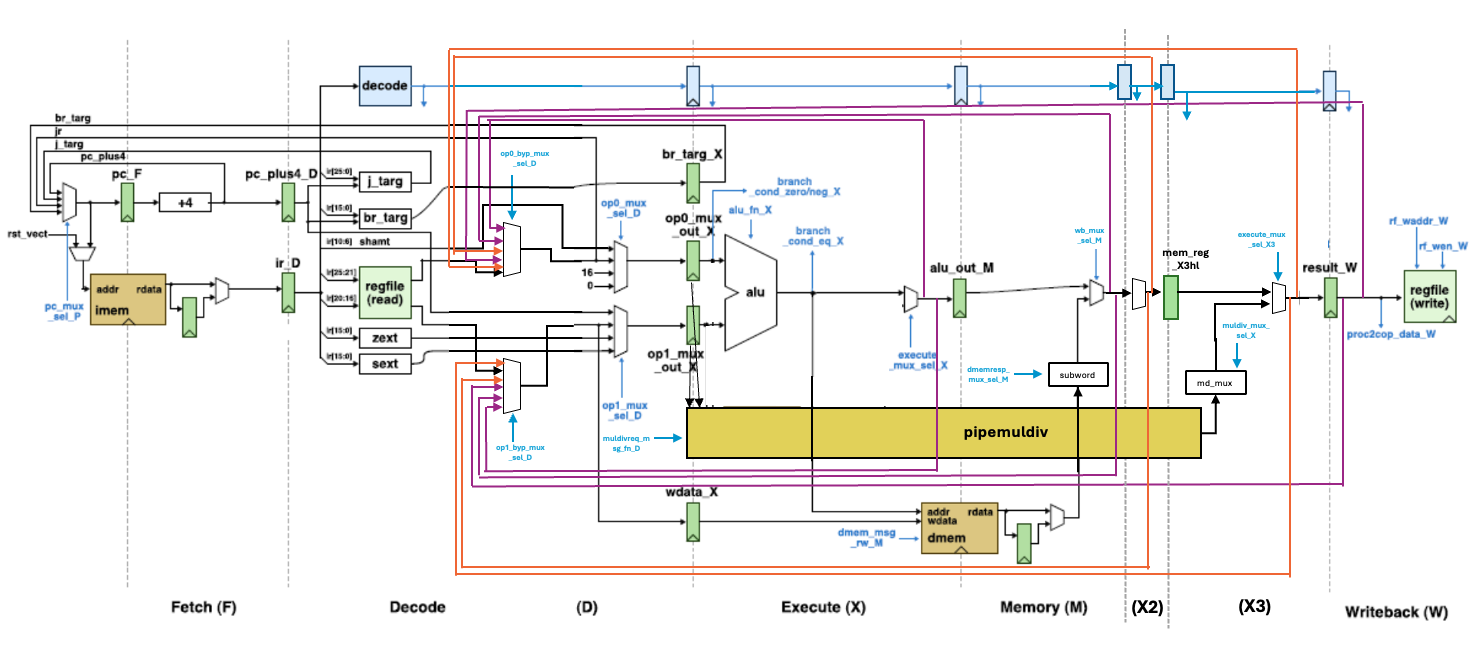
\includegraphics[scale=0.32]{./dualfetch-datapath.png}
\end{center}
Figure 1. Datapath of dualfetch processor from part 1.

\begin{center}
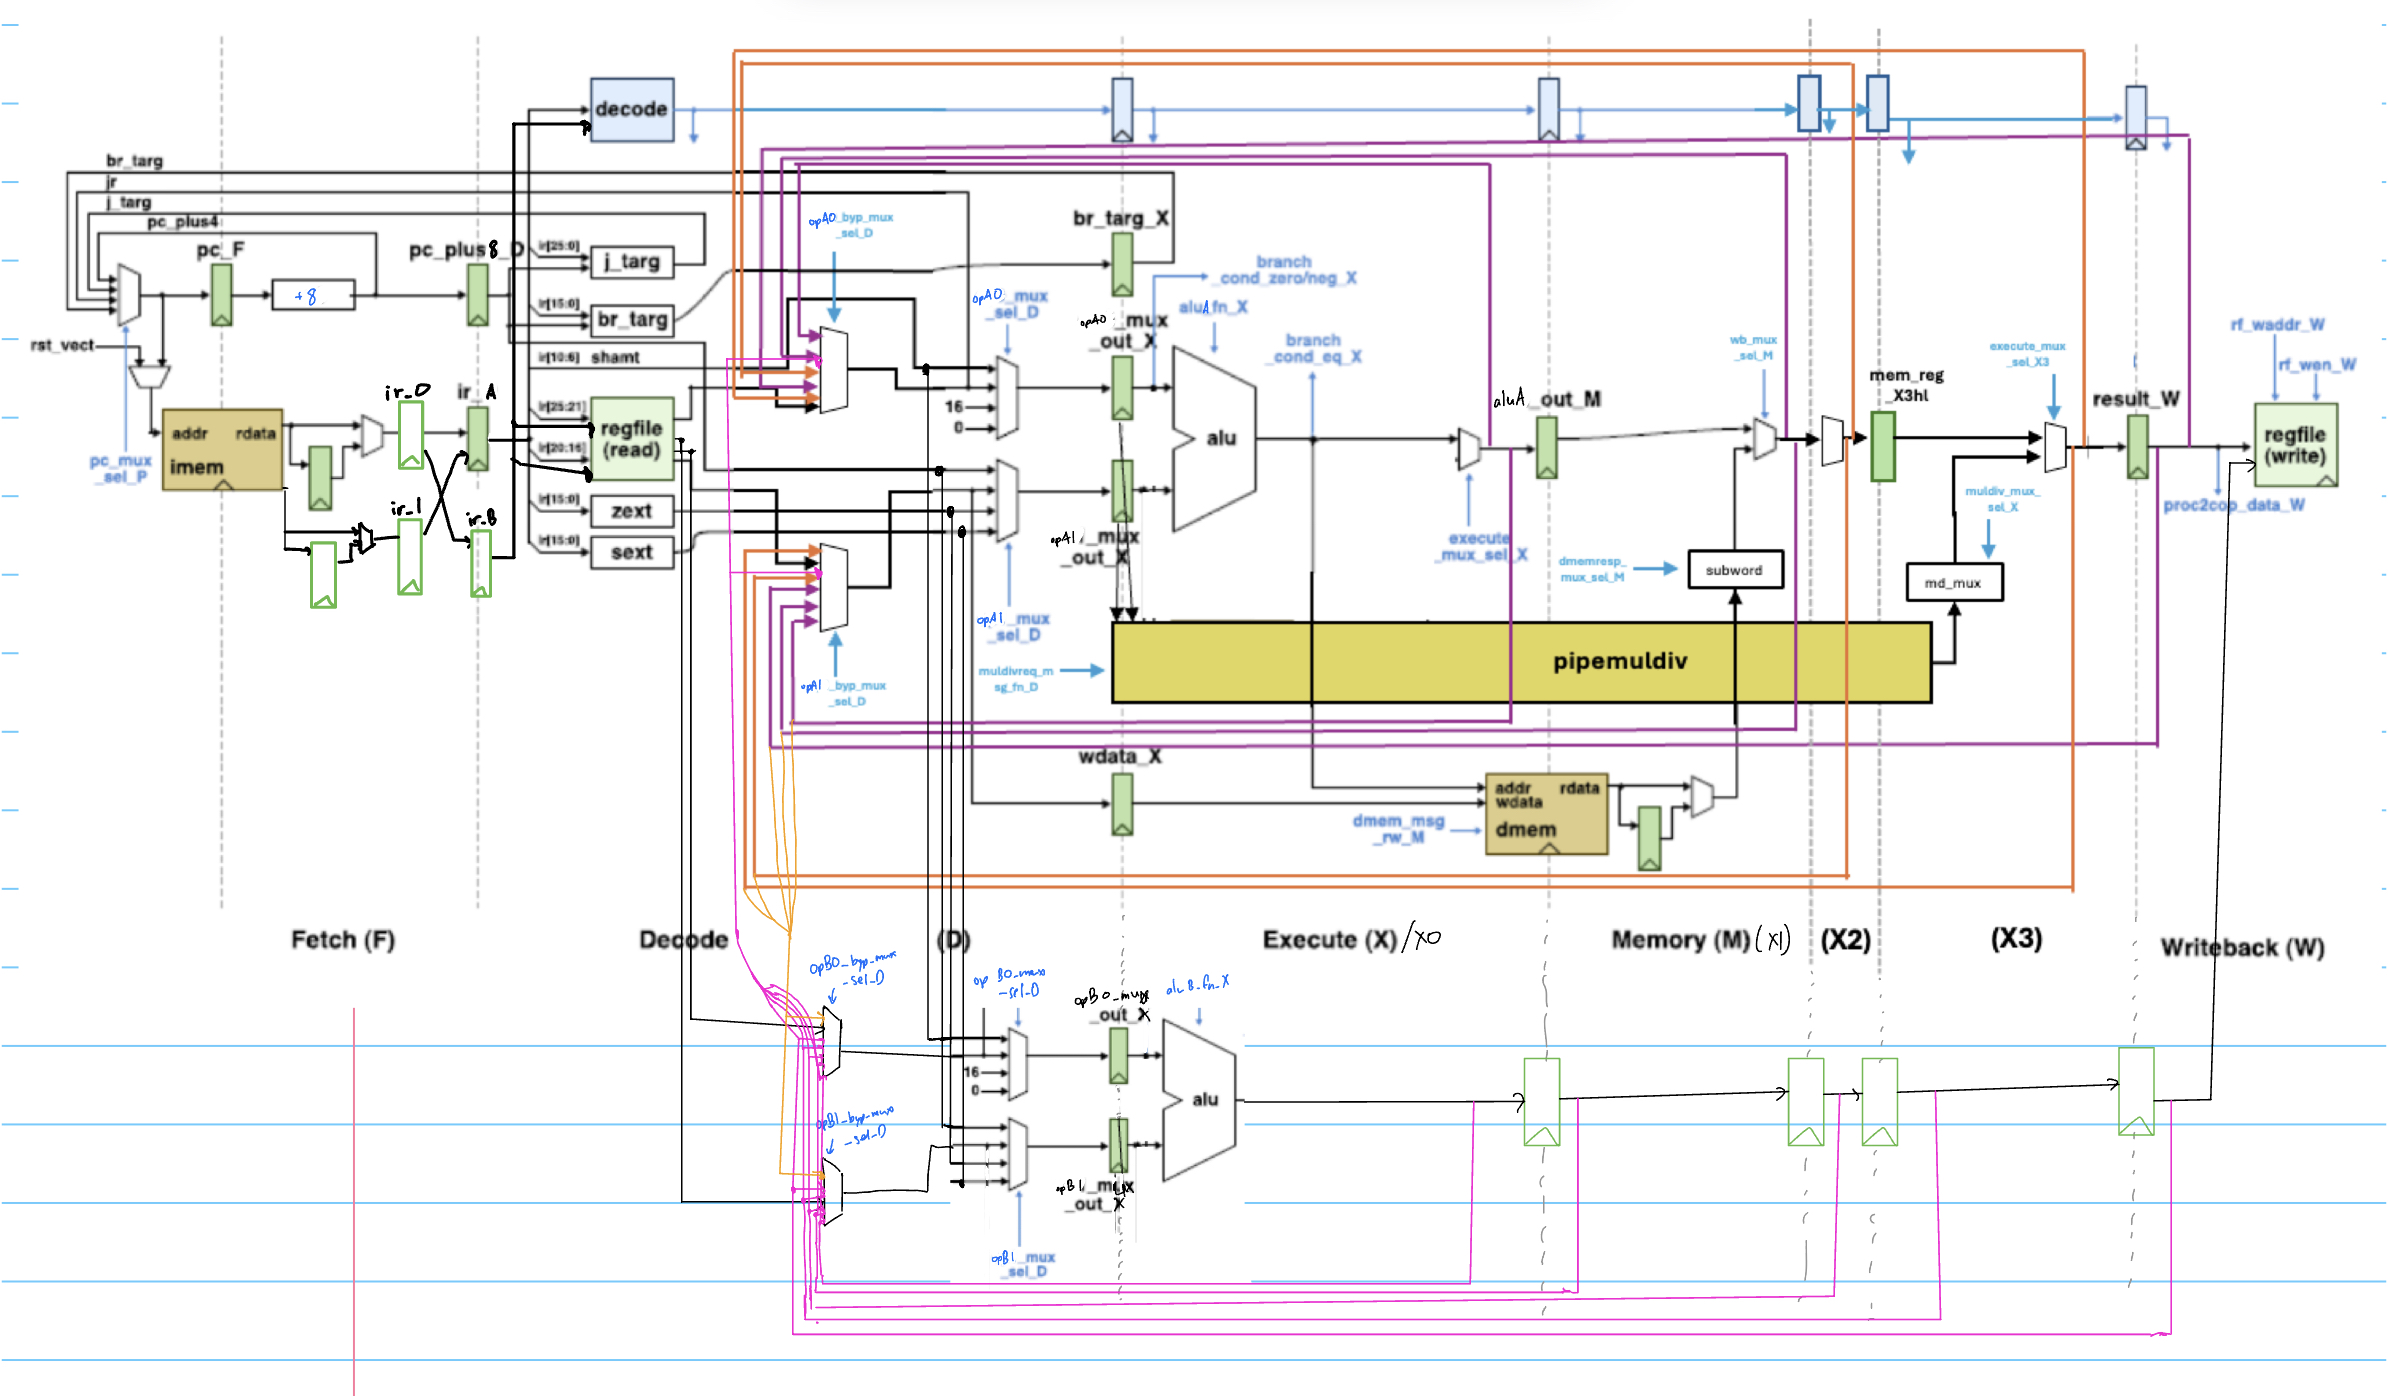
\includegraphics[scale=0.20]{./ssc-datapath.jpg}
\end{center}
Figure 2. Datapath of superscalar processor from part 2. \\

%See the new muxes within the Decode stage, one for op0 and one for op1. 

\begin{center}
    \begin{tabular}{|p{1in}| p{1in}| p{0.8in} | p{0.4in} | p{0.4in}| p{0.4in} | p{0.4in} | p{0.4in} |} 
 \hline
 Functional Unit[8] & Instruction Type[7:6] & Pending[5] & W[4] & X3[3] & X2[2] & X1[1]  & X0[0] \\
 \hline

\end{tabular}
\end{center}
Figure 3. Diagram of 9-bit wide scoreboard used in superscalar processor. \\



\end{document}


